\begin{center}
\begin{minipage}{0.45\textwidth}
\centering
\begin{tikzpicture}[
    every node/.style={
        circle, draw, minimum size=8mm,
        inner sep=0pt, outer sep=0pt
    },
    line width=0.7pt
]
    \path[use as bounding box]
        (-2,-1.1) rectangle (2,1.5);

    \node (u) at (0,0) {$u$};

    % Circular loop above the node
    \draw (u.60) arc[
        start angle=-60,
        end angle=240,
        radius=4mm
    ];
\end{tikzpicture}

\par\smallskip
Loop
\end{minipage}
\hfill
\begin{minipage}{0.45\textwidth}
\centering
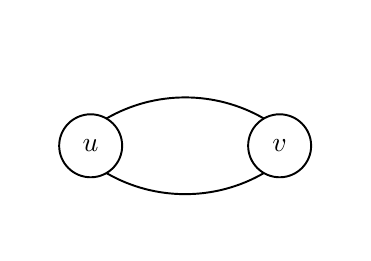
\begin{tikzpicture}[
    every node/.style={
        circle, draw, minimum size=8mm,
        inner sep=0pt, outer sep=0pt
    },
    line width=0.7pt
]
    \path[use as bounding box]
        (-2,-1.1) rectangle (2,1.5);

    \node (u) at (-1.2,0) {$u$};
    \node (v) at (1.2,0) {$v$};

    % Upper circular arc
    \draw (u.60) arc[
        start angle=120,
        end angle=60,
        radius=20mm
    ];

    % Lower circular arc
    \draw (u.-60) arc[
        start angle=240,
        end angle=300,
        radius=20mm
    ];
\end{tikzpicture}

\par\smallskip
Multiple Edges
\end{minipage}
\end{center}
